\documentclass[11pt,a4paper]{article}
\usepackage[utf8]{inputenc}
\usepackage{graphicx}
\graphicspath{ {images/}}
\begin{document}
\title{
Deliverable 1: Final Year Dissertation\\
\vspace{10mm}
Evolving a Learning Agent using Neuroevolution in the FightingICE Game Framework\\
\vspace{25mm}
}
\date{}
\author{Robert John Dunn\\
H00163867\\
BSc Honours in Computer Science\\
Heriot-Watt University\vspace{15mm}\\
Supervisor:\\
Dr Patricia A. Vargas\vspace{3mm}\\
Co-Supervisor:\\
Dr Fabrício Olivetti de França\vspace{3mm}\\
Second Reader:\\
Dr Mohamed Abdelshafy
}
\maketitle
\newpage
\vspace*{30mm}
\section*{Declaration}
I,  Robert Dunn confirm that this work submitted for assessment is my own and is expressed
in my own words. Any uses made within it of the works of other authors in any
form (e.g., ideas, equations, figures, text, tables, programs) are properly acknowledged
at any point of their use. A list of the references employed is included.\\
\\
Signed:\\
\\
Date: 
\newpage
\begin{abstract}
Neuroevolution is a popular technique for machine learning in which an artificial neural network is trained by an evolutionary algorithm. The technique take from the evolution of the biological nervous systems and is a popular approach for reinforcement learning problems. One way to demonstrate the effectiveness of neuroevolution is through artificial intelligence in games. This project aims to exercise neuroevolution techniques in order to evolve a learning agent in the FightingICE game framework. The agent is evolved with the goal of eventually being competitive versus a human opponent, and its performance will be evaluated at various stages of the evolution.
\end{abstract}
\newpage
\tableofcontents
\newpage
\section{Introduction}
\newpage
\section{Literature Review}
\subsection{Artificial Neural Networks}
\subsubsection{Fundamentals}
Artificial neural networks  
Neural networks are about associative memory or content-addressable memory. Neural networks are also about parallel processing.[book] 
Used for pattern 
What a perceptron is

\subsubsection{Activation Function}
More general nonlinear functions can be used. Usually required to saturate at -1 and +1. Tanhx (include image). \\
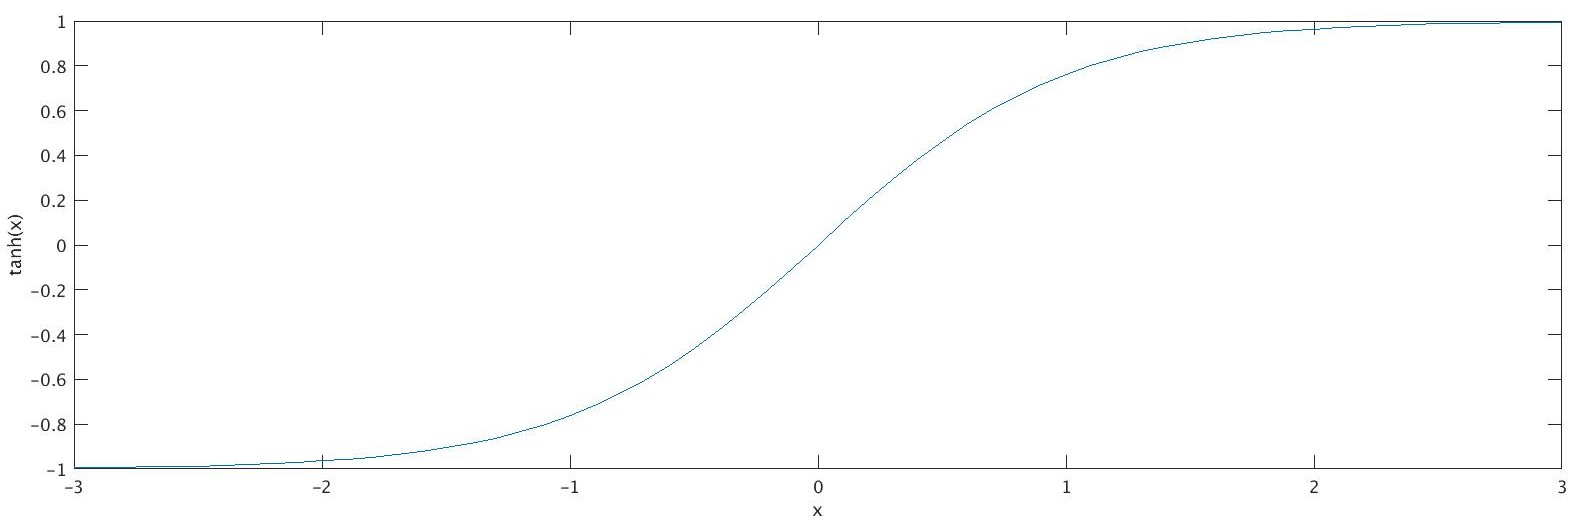
\includegraphics[width=\textwidth]{tanh}
Another possibility is to have neurons operate probabilistically. State is again +1 or -1 but now only a probability is given for the state to be -1 or +1.

\subsubsection{Network Training}
Multi-layer feed forward networks can learn by example, where the examples are inputs of which the outputs are known. This method of learning is called supervised learning. [book]
Neural networks are In order to train an artificial neural network, weights between neurons need to be adjusted in order to map th

\subsubsection{Biological Influence} 

\subsection{Machine Learning}

Artificial neural networks are 
\subsection{Neuroevolution}
Neuroevolution is a popular biologically-inspired method of machine learning in which an artificial neural network is evolved using an evolutionary algorithm. The popularity of the method stems from the fact that artificial intelligence and control problems can be cast as optimisation problems, and since the method is grounded in biological metaphor and evolutionary theory \cite{risi}.

What is neuroevolution and how it can be used for optimisation. ANNs evolving with EAs.

\subsubsection{Artificial Neural Networks}
What is an ANN. Different types of ANNs and benefits/drawbacks of each. Decisions which need to be made when implementing such as initial topology and weights.


\subsubsection{Evolutionary Algorithms}
How the EA alters the ANN, changing topology or weights. Types of EAs and pros/cons of each. How fitnesses are evaluated and mutation rate etc chosen.

\subsubsection{Performance of Neuroevolution}
Discuss how neuroevolution performs compared vs. other machine learning methods. Present success stories and any potential drawbacks/limitations.

\subsubsection{Neuroevolution in Games}
How neuroevolution can be used to evolve learning agents in games, usually agent is optimising some value e.g. HP. How fitness in games is evaluated, giving some examples. How neuroevolution fares compared to other learning algorithms. Present examples of projects implementing neuroevolution to learn.
\subsection{Machine Learning}
\subsubsection{Learning Paradigms}
Learning is an essential human function in which we modify our behaviour tendency according to experiences, to become better when a similar situation occurs. In the study of machine learning, algorithms, computer applications, and systems, utilise learning to improve their performance at certain tasks. There are two main entities in the machine learning model, the teacher and the learner. The teacher contains the knowledge to perform a given task while the learner has to learn 

\subsubsection{Incremental Evolution}

\newpage
\subsection{FightingICE}
\subsubsection{Game Framework}
What the FightingICE game is and details about the framework such as the language it's written in. Discuss reasons for choosing this over other possible frameworks/games.

\subsubsection{Game Agents}
Present information on the agents in the FightingICE game. The capabilities of the agents including which attack moves / movement commands they can do. Touch on fitness evaluation (how to win the game: keep enemy HP low and your HP high).

\subsubsection{Related Projects}
Discuss and reference relevant projects which have been completed using the FightingICE framework. Discuss what has been achieved in said projects and the potential further research that can be undertaken.

\newpage
\section{Requirements}

\section{Evaluation Strategy}

\section{Project Management}

\section{References}

[1] https://arxiv.org/pdf/1410.7326.pdf : Neuroevolution in Games: State of the Art and Open Challeng\\

[2] http://commerce3.derby.ac.uk/ojs/index.php/gb/article/view/3/1 : Improving AI for simulated cars using Neuroevolution\\

[3] http://commerce3.derby.ac.uk/ojs/index.php/gb/article/view/14/12 : Calculating Optimal Jungling Routes in DOTA2 Using Neural Networks and Genetic Algorithms\\

[4] https://www.cs.utexas.edu/~mhauskn/papers/atari.pdf : A Neuroevolution Approach to General Atari Game Playing\\

[5] https://arxiv.org/pdf/1512.01537v1.pdf : Reuse of Neural Modules for General Video Game Playing\\

http://www.cs.utexas.edu/users/nn/downloads/papers/gomez.ijcai99.pdf

https://arxiv.org/abs/1608.02971

https://arxiv.org/abs/1604.00644

https://arxiv.org/abs/1312.5355

https://arxiv.org/abs/1107.0037
http://nn.cs.utexas.edu/keyword?gomez:ab97
\section{Appendices}

\begin{thebibliography}{10}

\bibitem{risi}
	Risi, S \& Togelius, J.
	(2015).
	\emph{Neuroevolution in Games: State of the Art and Open Challenges},
  	[online],
  	Available at: https://arxiv.org/pdf/1410.7326.pdf
  	[Accessed 03 Nov. 2016]

\bibitem{pace}
	Pace, A. 
	(2014).
	\emph{Improving AI for simulated cars using Neuroevolution},
	[online],
	Available at: http://commerce3.derby.ac.uk/ojs/index.php/gb/article/view/3/1
	[Accessed 07 Nov. 2016]
	
\bibitem{lampro}
	Lampropoulos, A
	(2005)
	\emph{Machine Learning Paradigms.}
	Available at: \textit{http://file.allitebooks.com/20150722/Machine\%20Learning\%20Paradigms-\%20Applications\%20in\%20Recommender\%20Systems.pdf}
  

\end{thebibliography}
\end{document}